\documentclass[12pt]{article}

\usepackage[margin=1in, headheight=14.5pt]{geometry}
\usepackage{graphicx}
\usepackage{booktabs}
\usepackage{listings}
\usepackage{xcolor}
\usepackage{amsmath,amssymb}
\usepackage{caption}
\usepackage{float}
\usepackage{hyperref}
\usepackage{enumitem}
\usepackage{tabularx}
\usepackage{adjustbox}
\usepackage{fancyhdr}
\usepackage{titling}
\usepackage[numbers]{natbib}

\hypersetup{
  colorlinks=true,
  linkcolor=blue!60!black,
  urlcolor=blue!60!black,
  citecolor=blue!60!black,
}

% Page header/footer
\pagestyle{fancy}
\fancyhf{}
\fancyhead[L]{\small ECEC661 --- Homework 1}
\fancyhead[R]{\small Gary Pham (gp492)}
\fancyfoot[C]{\thepage}
\renewcommand{\headrulewidth}{0.4pt}

% VHDL listing style
\definecolor{vhdlkw}{RGB}{0,0,180}
\definecolor{vhdlcmt}{RGB}{0,128,0}
\definecolor{vhdlstr}{RGB}{160,0,0}
\definecolor{codebg}{RGB}{245,245,248}

\lstdefinelanguage{VHDL}{
  morekeywords=[1]{library,use,all,entity,is,generic,port,in,out,inout,
    end,architecture,of,begin,process,if,then,elsif,else,signal,
    variable,constant,type,range,downto,to,return,function,for,loop,
    natural,std_logic,std_logic_vector,unsigned,signed,rising_edge,
    report,severity,note,error,assert,wait,after,not,and,or,package,
    resize,others,map},
  morecomment=[l]{--},
  morestring=[b]",
  sensitive=false,
}

\lstset{
  language=VHDL,
  basicstyle=\ttfamily\footnotesize,
  keywordstyle=\color{vhdlkw}\bfseries,
  commentstyle=\color{vhdlcmt}\itshape,
  stringstyle=\color{vhdlstr},
  backgroundcolor=\color{codebg},
  frame=single,
  framerule=0.4pt,
  rulecolor=\color{gray!50},
  numbers=left,
  numberstyle=\tiny\color{gray},
  numbersep=6pt,
  breaklines=true,
  showstringspaces=false,
  tabsize=2,
  captionpos=b,
  aboveskip=8pt,
  belowskip=4pt,
}

% Title configuration
\pretitle{\begin{center}\LARGE\bfseries}
\posttitle{\par\end{center}\vskip 0.3em}

\title{ECEC661 --- Homework 1}
\author{Gary Pham --- gp492}
\date{\today}

\begin{document}
\maketitle
\thispagestyle{fancy}

% ======================================================================
\begin{abstract}
This report presents the design, implementation, and verification of three
digital circuits described in VHDL for ECEC661 Homework~1:
(1)~a combinational upper/lower output limiter (Problem~2.6.12),
(2)~a sequential synchronous palindrome checker (Problem~3.5.11), and
(3)~an accumulator built around a Vivado IP core (Problem~7.5.3).
Each design is accompanied by a self-checking testbench that applies
stimulus vectors and automatically verifies expected outputs via VHDL
\texttt{assert} statements. Waveform results are captured from Xilinx
XSim~\cite{ug900} simulation in batch mode through VCD export and
plotted with Python. All simulations pass with zero assertion errors.
\end{abstract}

% ======================================================================
\section{Introduction}
\label{sec:intro}
% ======================================================================

Hardware description languages such as VHDL~\cite{ieee1076} enable
designers to specify digital circuits at the register-transfer level (RTL)
and verify them through simulation before committing to silicon or FPGA
implementation. This report documents three exercises that cover a range
of fundamental HDL design patterns:

\begin{itemize}[nosep]
  \item \textbf{Combinational logic} --- the output limiter uses a purely
        combinational process with unsigned comparisons to clamp an input
        within a parameterised range (Section~\ref{sec:limiter}).
  \item \textbf{Synchronous sequential logic} --- the palindrome checker
        uses clocked shift registers and a bit-reversal comparison to
        determine whether two serially received bit-streams form a
        palindrome pair (Section~\ref{sec:palindrome}).
  \item \textbf{IP integration} --- the accumulator wraps a Vivado
        Accumulator IP core (or a portable behavioural stand-in) within
        a simple top-level entity, demonstrating hierarchical design and
        IP reuse (Section~\ref{sec:accumulator}).
\end{itemize}

\noindent
All designs target Xilinx Vivado 2025.2~\cite{ug900} and are simulated
with the included XSim simulator. Section~\ref{sec:methodology}
describes the simulation and verification methodology, followed by
dedicated sections for each design. Section~\ref{sec:conclusion}
summarises the results.

% ======================================================================
\section{Simulation and Verification Methodology}
\label{sec:methodology}
% ======================================================================

Each design is paired with a self-checking VHDL testbench. The
testbenches share a common verification strategy:

\begin{enumerate}[nosep]
  \item \textbf{Stimulus generation.} The testbench drives input signals
        according to a predefined sequence (either exhaustive or
        selected corner cases).
  \item \textbf{Automated checking.} After each stimulus application
        (and appropriate settling or clock-edge wait), a VHDL
        \texttt{assert} statement compares the DUT output against the
        analytically expected value. Any mismatch raises an
        \texttt{error}-severity message.
  \item \textbf{Pass/fail reporting.} Upon completing all vectors
        without error, the testbench prints a
        ``\texttt{<testbench\_name> PASSED}'' note and terminates
        via \texttt{std.env.stop}.
\end{enumerate}

\noindent
Waveforms are captured in batch mode (no GUI) by elaborating with
\texttt{xelab~\ldots~-debug typical} to enable trace information,
then running XSim with a Tcl script that calls \texttt{open\_vcd},
\texttt{log\_vcd}, and \texttt{close\_vcd}~\cite{ug900}.
The resulting IEEE~1364 VCD files~\cite{ieee1364} are parsed and plotted
with Python (\texttt{vcdvcd} and \texttt{matplotlib}).
Table~\ref{tab:manifest} lists the deliverables for each problem.

\begin{table}[H]
\centering
\caption{File manifest for each homework problem.}
\label{tab:manifest}
\begin{adjustbox}{max width=\textwidth}
\begin{tabular}{@{}llll@{}}
\toprule
\textbf{Problem} & \textbf{Design Source} & \textbf{Testbench} & \textbf{Waveform} \\
\midrule
2.6.12 Output Limiter
  & \texttt{output\_limiter.vhd}
  & \texttt{tb\_output\_limiter.vhd}
  & \texttt{waveform\_limiter.png} \\[4pt]
3.5.11 Palindrome Checker
  & \texttt{palindrome\_synch\_ckt.vhd}
  & \texttt{tb\_palindrome\_synch\_ckt.vhd}
  & \texttt{waveform\_palindrome.png} \\[4pt]
7.5.3 Accumulator IP
  & \texttt{accumulator\_top.vhd}, \texttt{c\_accum\_0.vhd}
  & \texttt{tb\_accumulator\_top.vhd}
  & \texttt{waveform\_accumulator.png} \\
\bottomrule
\end{tabular}
\end{adjustbox}
\end{table}

% ======================================================================
\section{Problem 2.6.12 --- Upper and Lower Output Limiter}
\label{sec:limiter}
% ======================================================================

\subsection{Problem Statement}

Design a combinational circuit that receives an $n$-bit unsigned input
$x$ and produces an output $z$ clamped between a lower limit~$l$ and an
upper limit~$u$. Both limits are configurable via VHDL generics.
Formally:
\begin{equation}
  z = \begin{cases}
        l & \text{if } x < l,\\
        u & \text{if } x > u,\\
        x & \text{otherwise.}
      \end{cases}
  \label{eq:limiter}
\end{equation}

\subsection{Design Description}

The implementation consists of a package \texttt{output\_limiter} that
declares the bit-width constant $n = 4$, and an entity
\texttt{user\_logic} parameterised by generics \texttt{u} and
\texttt{l} (both $n$-bit vectors, defaulting to all-ones and all-zeros,
respectively). The architecture contains a single sensitivity-list
process that evaluates the unsigned comparisons in
Equation~\eqref{eq:limiter} using the \texttt{IEEE.NUMERIC\_STD}
\texttt{unsigned} type~\cite{ieee1076}.

Since the process is purely combinational (the sensitivity list contains
only the input \texttt{x} and there are no clock or storage elements),
synthesis tools will infer a comparator--multiplexer chain with no
registers.

\subsection{Source Code}
\lstinputlisting[caption={output\_limiter.vhd --- Package and entity for the output limiter.}]{output_limiter.vhd}

\subsection{Testbench Design}
\label{sec:limiter:tb}

The testbench \texttt{tb\_output\_limiter} instantiates
\texttt{user\_logic} with $u = \texttt{"1010"}$ (decimal~10) and
$l = \texttt{"0101"}$ (decimal~5). It performs an \emph{exhaustive}
sweep of all $2^n = 16$ input values ($x = 0, 1, \ldots, 15$) with a
10\,ns settling delay between each. At every step, the expected output
is computed in a VHDL variable and compared against the DUT output
\texttt{z} using an \texttt{assert} statement.

The exhaustive approach guarantees that every possible input combination
is tested --- a practical strategy for small bit-widths. For larger
designs, a corner-case strategy would be more appropriate.

\lstinputlisting[caption={tb\_output\_limiter.vhd --- Exhaustive self-checking testbench.}]{tb_output_limiter.vhd}

\subsection{Simulation Waveform}

\begin{figure}[H]
  \centering
  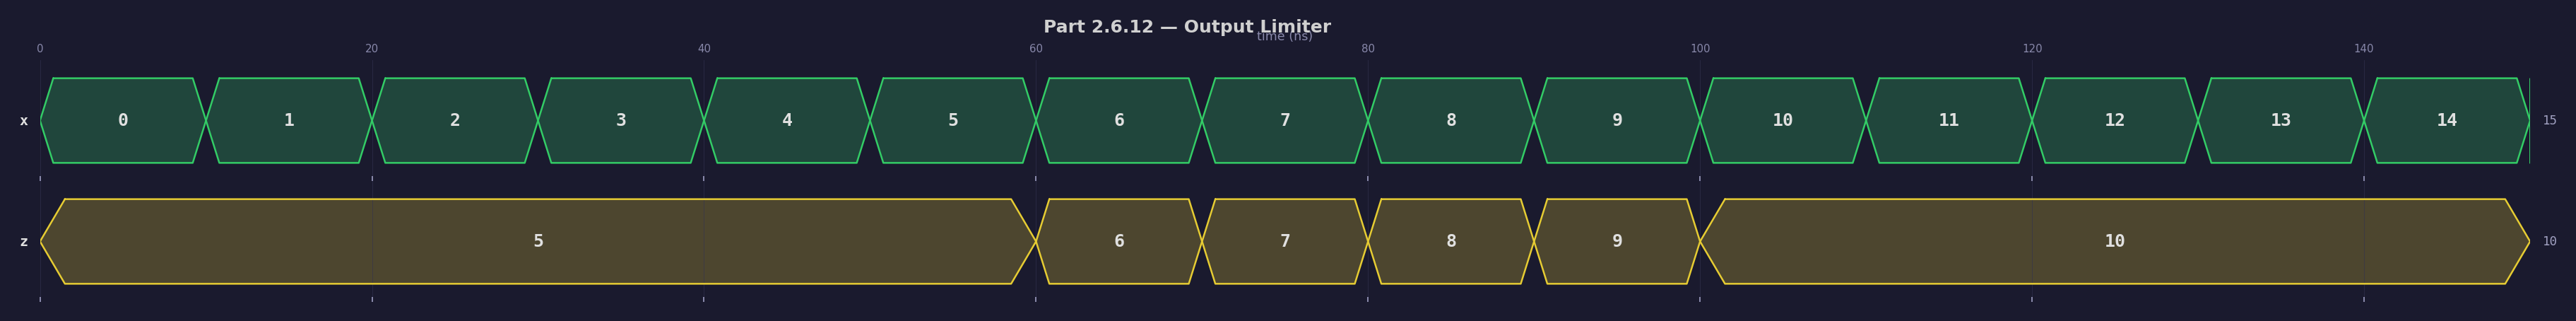
\includegraphics[width=\textwidth]{waveform_limiter.png}
  \caption{Output Limiter waveform: \texttt{x} sweeps 0--15 while
           \texttt{z} is clamped between 5 and 10.}
  \label{fig:limiter}
\end{figure}

\subsection{Results and Discussion}

Table~\ref{tab:limiter_results} summarises the observed clamping
behaviour across the three distinct input regions.

\begin{table}[H]
\centering
\caption{Output limiter verification summary ($l=5$, $u=10$).}
\label{tab:limiter_results}
\begin{tabular}{@{}ccl@{}}
\toprule
\textbf{Input range} & \textbf{Expected $z$} & \textbf{Observed behaviour} \\
\midrule
$x \in [0, 4]$    & 5 (lower limit)  & $z$ remains constant at 5 \\
$x \in [5, 10]$   & $x$ (pass-through) & $z$ tracks $x$: 5, 6, 7, 8, 9, 10 \\
$x \in [11, 15]$  & 10 (upper limit) & $z$ remains constant at 10 \\
\bottomrule
\end{tabular}
\end{table}

\noindent
The simulation log confirms: \texttt{tb\_output\_limiter PASSED} with
zero assertion errors, verifying functional correctness for every
possible 4-bit input.

% ======================================================================
\section{Problem 3.5.11 --- Sequential Palindrome Checker}
\label{sec:palindrome}
% ======================================================================

\subsection{Problem Statement}

Design a synchronous sequential circuit that receives two serial
bit-streams $x$ and $y$ (one bit per clock cycle, LSB first) and, after
$n$~clock cycles, asserts output $z$ if the accumulated $x$~vector
equals the bit-reversal of the accumulated $y$~vector:
\begin{equation}
  z = \begin{cases}
        1 & \text{if } X[n{-}1:0] = \operatorname{reverse}(Y[n{-}1:0]),\\
        0 & \text{otherwise.}
      \end{cases}
  \label{eq:palindrome}
\end{equation}

\subsection{Design Description}

Entity \texttt{palindrome\_synch\_ckt} is parameterised by
generic $n$ (default~5). Internally, two $n$-bit shift registers
(\texttt{x\_shift}, \texttt{y\_shift}) and a counter \texttt{count}
track how many bits have been captured since the last reset. On each
rising clock edge:

\begin{itemize}[nosep]
  \item If \texttt{reset = '1'}: all registers and the output are
        cleared to zero.
  \item If \texttt{count $<$ n}: the current input bits are shifted into
        the LSB of the respective registers, and \texttt{count} is
        incremented.
  \item When \texttt{count} reaches $n - 1$ (i.e.\ the $n$-th sample is
        being captured in the same clock cycle): the comparison
        $\texttt{x\_next} \stackrel{?}{=}
        \operatorname{reverse}(\texttt{y\_next})$ is evaluated on the
        \emph{about-to-be-latched} values via local variables, ensuring
        the result is available one clock edge after the last input.
\end{itemize}

\noindent
A helper function \texttt{reverse\_bits} performs a compile-time-known
loop reversal of a \texttt{std\_logic\_vector}, which synthesises to
wire re-ordering (zero logic cost)~\cite{pedroni2010}.

\subsection{Source Code}
\lstinputlisting[caption={palindrome\_synch\_ckt.vhd --- Synchronous palindrome checker.}]{palindrome_synch_ckt.vhd}

\subsection{Testbench Design}
\label{sec:palindrome:tb}

The testbench \texttt{tb\_palindrome\_synch\_ckt} exercises two
back-to-back scenarios with $n = 5$, separated by a reset pulse:

\paragraph{Test~1 --- Palindrome match.}
\begin{itemize}[nosep]
  \item $x$ sequence: 1, 0, 1, 0, 1 $\;\Rightarrow\; X = \texttt{10101}$.
  \item $y$ sequence: 1, 0, 1, 0, 1 $\;\Rightarrow\; Y = \texttt{10101}$.
  \item $\operatorname{reverse}(Y) = \texttt{10101} = X$, hence $z$
        should be~\texttt{'1'}.
\end{itemize}

\paragraph{Test~2 --- Non-palindrome.}
\begin{itemize}[nosep]
  \item $x$ sequence: 1, 1, 0, 0, 1 $\;\Rightarrow\; X = \texttt{11001}$.
  \item $y$ sequence: 1, 0, 1, 0, 0 $\;\Rightarrow\; Y = \texttt{10100}$.
  \item $\operatorname{reverse}(Y) = \texttt{00101} \neq X$, hence $z$
        should be~\texttt{'0'}.
\end{itemize}

\noindent
The testbench asserts the expected $z$ value one clock cycle after the
final input of each test, then reports pass/fail.

\lstinputlisting[caption={tb\_palindrome\_synch\_ckt.vhd --- Two-case self-checking testbench.}]{tb_palindrome_synch_ckt.vhd}

\subsection{Simulation Waveform}

\begin{figure}[H]
  \centering
  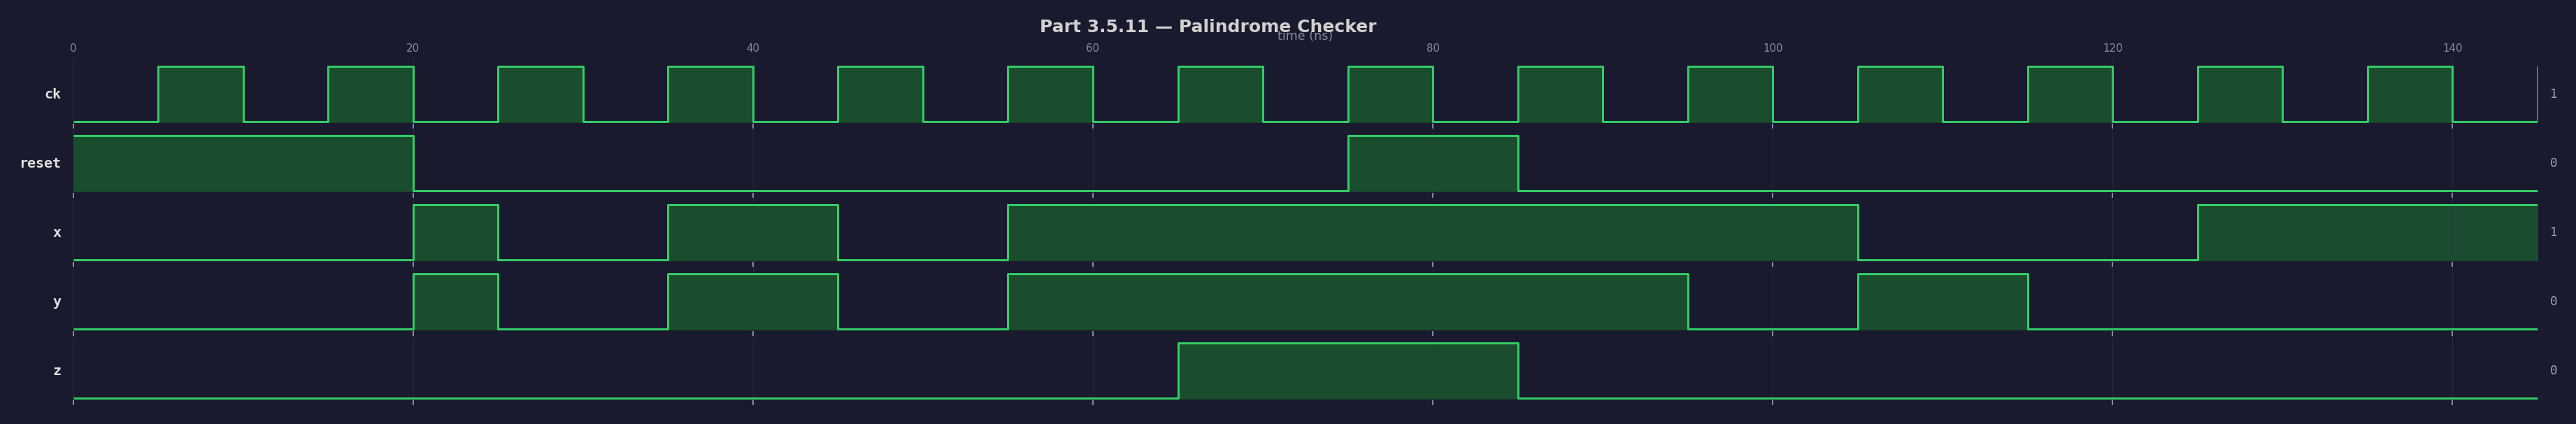
\includegraphics[width=\textwidth]{waveform_palindrome.png}
  \caption{Palindrome Checker waveform: Test~1 produces $z=1$
           (palindrome match); Test~2 produces $z=0$ (no match).}
  \label{fig:palindrome}
\end{figure}

\subsection{Results and Discussion}

The waveform in Figure~\ref{fig:palindrome} shows two distinct test
windows separated by a reset pulse:

\begin{enumerate}[nosep]
  \item \textbf{First window ($t \approx 20$--$70$\,ns):} After five
        clock cycles of input capture, \texttt{z} rises to~\texttt{'1'},
        confirming the palindrome match between
        $X = \texttt{10101}$ and
        $\operatorname{reverse}(Y) = \texttt{10101}$.
  \item \textbf{Second window ($t \approx 80$--$130$\,ns):} After five
        more clock cycles with different inputs, \texttt{z} remains
        at~\texttt{'0'}, confirming the non-palindrome case where
        $X = \texttt{11001}$ differs from
        $\operatorname{reverse}(Y) = \texttt{00101}$.
\end{enumerate}

\noindent
The simulation log reports \texttt{tb\_palindrome\_synch\_ckt PASSED}
with zero assertion errors.

% ======================================================================
\section{Problem 7.5.3 --- Accumulator IP and Testbench}
\label{sec:accumulator}
% ======================================================================

\subsection{Problem Statement}

Using the Vivado IP Catalog, generate an Accumulator IP core configured
for 4-bit signed input and 8-bit signed output with synchronous clear.
Wrap the IP in a top-level entity and write a testbench that verifies
correct accumulation over a sequence of signed inputs.

\subsection{Design Description}

The design is structured as a two-level hierarchy:

\begin{enumerate}[nosep]
  \item \textbf{\texttt{accumulator\_top}} --- a thin RTL wrapper that
        exposes ports \texttt{ck} (clock), \texttt{sclr} (synchronous
        clear), \texttt{x} (4-bit signed input), and \texttt{q} (8-bit
        signed output). It instantiates the accumulator IP via direct
        entity instantiation.
  \item \textbf{\texttt{c\_accum\_0}} --- the accumulator core. Two
        interchangeable implementations exist:
        \begin{itemize}[nosep]
          \item \emph{Vivado IP:} Generated from the IP Catalog
                (\texttt{Accumulator} category); configured for 4-bit
                signed input, 8-bit signed output, with synchronous
                clear~\cite{pg119}.
          \item \emph{Behavioural stand-in:} A portable VHDL model
                (\texttt{c\_accum\_0.vhd}) with identical port names
                (\texttt{B}, \texttt{CLK}, \texttt{SCLR}, \texttt{Q})
                and identical semantics. This allows simulation without
                requiring IP generation.
        \end{itemize}
\end{enumerate}

\noindent
On each rising clock edge: if $\texttt{SCLR} = 1$, the internal
accumulator register resets to zero; otherwise, the 4-bit signed input
is sign-extended to 8~bits and added to the running sum:
\begin{equation}
  Q^{(k)} = \begin{cases}
              0 & \text{if SCLR} = 1, \\
              Q^{(k-1)} + \operatorname{sign\_ext}(B, 8) & \text{otherwise.}
             \end{cases}
  \label{eq:accum}
\end{equation}

\subsection{Source Code}

\lstinputlisting[caption={accumulator\_top.vhd --- Top-level IP wrapper.}]{accumulator_top.vhd}
\lstinputlisting[caption={c\_accum\_0.vhd --- Behavioural stand-in for the Vivado Accumulator IP.}]{c_accum_0.vhd}

\subsection{Testbench Design}
\label{sec:accumulator:tb}

The testbench \texttt{tb\_accumulator\_top} applies a sequence of 20
signed 4-bit values spanning the full representable range
$[-8, +7]$ plus selected mixed-sign values:

\begin{center}
\small
\texttt{-8, -7, -6, -5, -4, -3, -2, -1, 0, 1, 2, 3, 4, 5, 6, 7, -8, 7, -1, 6}
\end{center}

\noindent
The verification procedure is:
\begin{enumerate}[nosep]
  \item Assert synchronous clear: pulse \texttt{sclr} high for one
        clock cycle, then verify $q = 0$.
  \item For each of the 20 input samples: drive \texttt{x}, wait for one
        rising clock edge plus 1\,ns propagation, then assert that
        \texttt{q} equals the analytically computed running sum using a
        VHDL variable \texttt{expected\_sum}.
  \item Report \texttt{PASSED} upon completion.
\end{enumerate}

\lstinputlisting[caption={tb\_accumulator\_top.vhd --- 20-sample self-checking testbench.}]{tb_accumulator_top.vhd}

\paragraph{Expected running-sum trace.}
Table~\ref{tab:accum_trace} shows the analytically derived running sum
at each sample, which the testbench verifies cycle-by-cycle.

\begin{table}[H]
\centering
\caption{Accumulator expected running-sum trace ($\Sigma$ is the
         cumulative sum after sample $\#$).}
\label{tab:accum_trace}
\begin{tabular}{@{}rrr@{\qquad}rrr@{\qquad}rrr@{\qquad}rrr@{}}
\toprule
\textbf{\#} & \textbf{x} & $\boldsymbol{\Sigma}$
& \textbf{\#} & \textbf{x} & $\boldsymbol{\Sigma}$
& \textbf{\#} & \textbf{x} & $\boldsymbol{\Sigma}$
& \textbf{\#} & \textbf{x} & $\boldsymbol{\Sigma}$ \\
\midrule
0  & $-8$ & $-8$  & 5  & $-3$ & $-33$ & 10 & 2  & $-33$ & 15 & 7    & $-8$  \\
1  & $-7$ & $-15$ & 6  & $-2$ & $-35$ & 11 & 3  & $-30$ & 16 & $-8$ & $-16$ \\
2  & $-6$ & $-21$ & 7  & $-1$ & $-36$ & 12 & 4  & $-26$ & 17 & 7    & $-9$  \\
3  & $-5$ & $-26$ & 8  & 0    & $-36$ & 13 & 5  & $-21$ & 18 & $-1$ & $-10$ \\
4  & $-4$ & $-30$ & 9  & 1    & $-35$ & 14 & 6  & $-15$ & 19 & 6    & $-4$  \\
\bottomrule
\end{tabular}
\end{table}

\subsection{Simulation Waveform}

\begin{figure}[H]
  \centering
  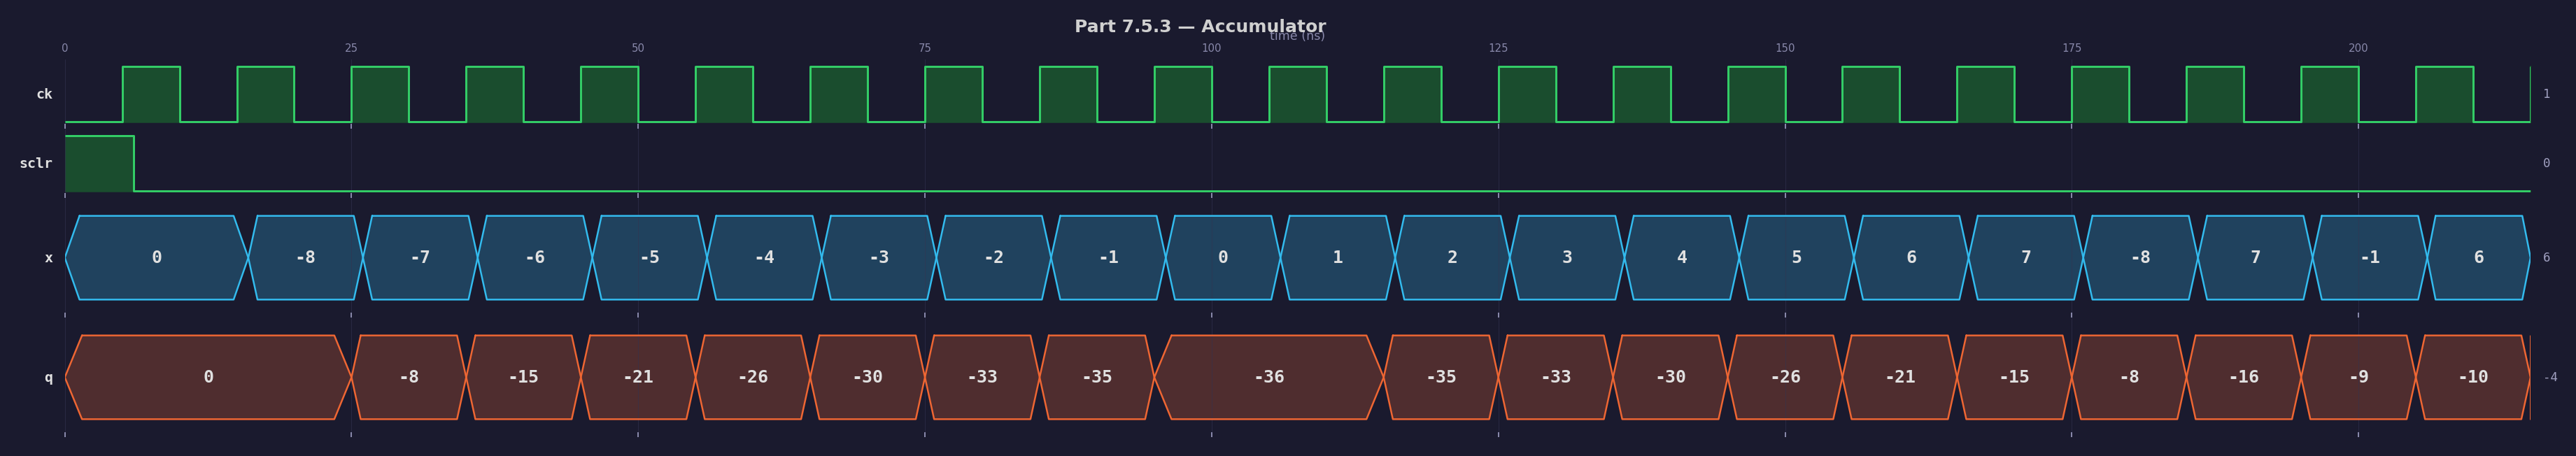
\includegraphics[width=\textwidth]{waveform_accumulator.png}
  \caption{Accumulator waveform: \texttt{x} shows each signed 4-bit
           input; \texttt{q} shows the 8-bit running sum matching
           Table~\ref{tab:accum_trace}.}
  \label{fig:accumulator}
\end{figure}

\subsection{Results and Discussion}

The waveform in Figure~\ref{fig:accumulator} confirms correct operation:

\begin{enumerate}[nosep]
  \item \textbf{Synchronous clear:} After the initial \texttt{sclr}
        pulse, \texttt{q} is zero as expected.
  \item \textbf{Accumulation accuracy:} The \texttt{q} trace matches
        the expected running sum in Table~\ref{tab:accum_trace}. The sum
        descends to $-36$ during samples~0--8 (all negative or zero
        inputs), then rises as positive values are added during
        samples~9--15, and finally settles at $-4$ after the last four
        mixed-sign inputs.
  \item \textbf{Signed arithmetic:} The accumulator correctly handles
        two's complement sign extension from 4 bits to 8 bits (via
        \texttt{resize(signed(B),\,8)} in the behavioural model)
        throughout the entire sequence.
\end{enumerate}

\noindent
The simulation log reports \texttt{tb\_accumulator\_top PASSED} with
zero assertion errors across all 20 samples plus the clear check.

\subsection{IP Portability Note}

On a Vivado-equipped machine, the Vivado IP Catalog \texttt{c\_accum\_0}
core can be generated and will seamlessly replace the behavioural
\texttt{c\_accum\_0.vhd}. The port interface (\texttt{B}, \texttt{CLK},
\texttt{SCLR}, \texttt{Q}) and accumulation semantics are
identical~\cite{pg119}. The behavioural stand-in is provided for
portable simulation without requiring IP generation.

% ======================================================================
\section{Conclusion}
\label{sec:conclusion}
% ======================================================================

Three VHDL designs were implemented and verified through self-checking
testbenches simulated in Xilinx XSim:

\begin{itemize}[nosep]
  \item The \textbf{output limiter} correctly clamps unsigned inputs
        within the parameterised bounds, verified exhaustively over all
        $2^4 = 16$ input values.
  \item The \textbf{palindrome checker} correctly identifies palindrome
        and non-palindrome serial bit-stream pairs, verified across two
        representative test cases with reset separation.
  \item The \textbf{accumulator} correctly computes a signed running sum
        with synchronous clear, verified against 20 analytically derived
        expected values.
\end{itemize}

\noindent
All three testbenches report \texttt{PASSED} with zero assertion errors,
confirming functional correctness of each design.

% ======================================================================
% References
% ======================================================================
\bibliographystyle{ieeetr}

\begin{thebibliography}{9}

\bibitem{ug900}
AMD/Xilinx, ``Vivado Design Suite User Guide: Logic Simulation
(UG900),'' v2025.2, 2025.
\url{https://docs.amd.com/r/en-US/ug900-vivado-logic-simulation}

\bibitem{ieee1076}
IEEE, ``IEEE Standard VHDL Language Reference Manual,'' IEEE Std
1076-2008, 2009.

\bibitem{ieee1364}
IEEE, ``IEEE Standard for Verilog Hardware Description Language ---
Value Change Dump (VCD),'' IEEE Std 1364-2005, Sec.~18, 2006.

\bibitem{pg119}
AMD/Xilinx, ``Accumulator (PG119),'' LogiCORE IP Product Guide, v12.0,
2015.
\url{https://docs.amd.com/v/u/en-US/pg119-c-accum}

\bibitem{pedroni2010}
V.~A.~Pedroni, \textit{Circuit Design and Simulation with VHDL}, 2nd
ed.\@ MIT Press, 2010.

\end{thebibliography}

\end{document}
